%%%%%%%%%%%%%%%%%%%%%%%%%%%%%%%%%%%%%%%%%%%%%%%%%%%%%%%%%%%%%%%%%%%%%%%%
%%%%%%%%%%%%%%%%%%%%%%%%%%%%%%%%%%%%%%%%%%%%%%%%%%%%%%%%%%%%%%%%%%%%%%%%
\documentclass[12pt,a4paper,oneside]{scrreprt}
\usepackage[utf8]{inputenc}
%\usepackage[ngerman]{babel}
\usepackage{units,tabularx,lipsum,longtable}
\usepackage[table]{xcolor}
\usepackage[margin=2cm]{geometry}
\usepackage[green,extramargin,bcor=1.2cm]{tubsdoc}
\defbglayout[sender=top,pages=single]{newlayout}{ %
\showtubslogo[left] 	%	TUBS-Logo
%\showtopline 			%	Rote Linie oben
}
\logo{
\includegraphics{./images/logo/InA-TECH-elPaSo-rgb.pdf}}
\usepackage[htt]{hyphenat}
\usepackage[obeyspaces]{url} %Darstellung der Dateipfade und Programmiercode im Fließtext
\expandafter\def\expandafter\UrlBreaks\expandafter{\UrlBreaks%  save the current one
  \do\a\do\b\do\c\do\d\do\e\do\f\do\g\do\h\do\i\do\j%
  \do\k\do\l\do\m\do\n\do\o\do\p\do\q\do\r\do\s\do\t%
  \do\u\do\v\do\w\do\x\do\y\do\z\do\A\do\B\do\C\do\D%
  \do\E\do\F\do\G\do\H\do\I\do\J\do\K\do\L\do\M\do\N%
  \do\O\do\P\do\Q\do\R\do\S\do\T\do\U\do\V\do\W\do\X%
  \do\Y\do\Z}
\usepackage{listings} %Programmiercode darstellen
\usepackage{amssymb, mathtools}
\usepackage{enumitem}
\renewcommand{\tt}{\ttfamily}

%netbeans coloring style for C++
\definecolor{dkgreen}{rgb}{0,0.6,0}
\lstset{frame={},
  language=C++,
  aboveskip=3mm,
  belowskip=3mm,
  showstringspaces=false,
  columns=flexible,
  basicstyle={\small\ttfamily},
  numbers=none,
  numberstyle=\tiny\color{black},  
  keywordstyle=\color{blue},
  commentstyle=\color{gray},
  stringstyle=\color{orange},
  breaklines=true,
  breakatwhitespace=true,
  tabsize=3,
  %define new color style for member variables
  moredelim=[is][\color{dkgreen}]{$m:}{:m$},
  %define new color style for define keywords
  moredelim=[s][\color{green}]{\#{}ifndef}{\ },
  moredelim=[s][\color{green}]{\#{}define}{\ },
  moredelim=[s][\color{green}]{\#{}endif}{\ },
}

\usepackage{multirow}
\usepackage{adjustbox}

\usepackage{float}
\usepackage{longtable}
\usepackage[backend=bibtex,style=numeric,natbib=true, maxbibnames=99]{biblatex}
\bibliography{literature/keypubelpaso}

\begin{document}
\parindent 0pt
\title{elPaSo-Core Manual}
\date{\the\year{}}
\author{\Large Institute for Acoustics, Technische Universität Braunschweig}
\maketitle
\pagenumbering{roman}
\tableofcontents
\cleardoublepage
%\normalem
\pagenumbering{arabic}

\chapter{Introduction}

\section{About elPaSo}

The research code “Elementary Parallel Solver (elPaSo)” is the in-house vibroacoustic simulation tool constantly developed over 25 years at TU Braunschweig, presently extended and maintained by the Institute for Acoustics (InA), TU Braunschweig.

\begin{figure}[h!]
    \centering
    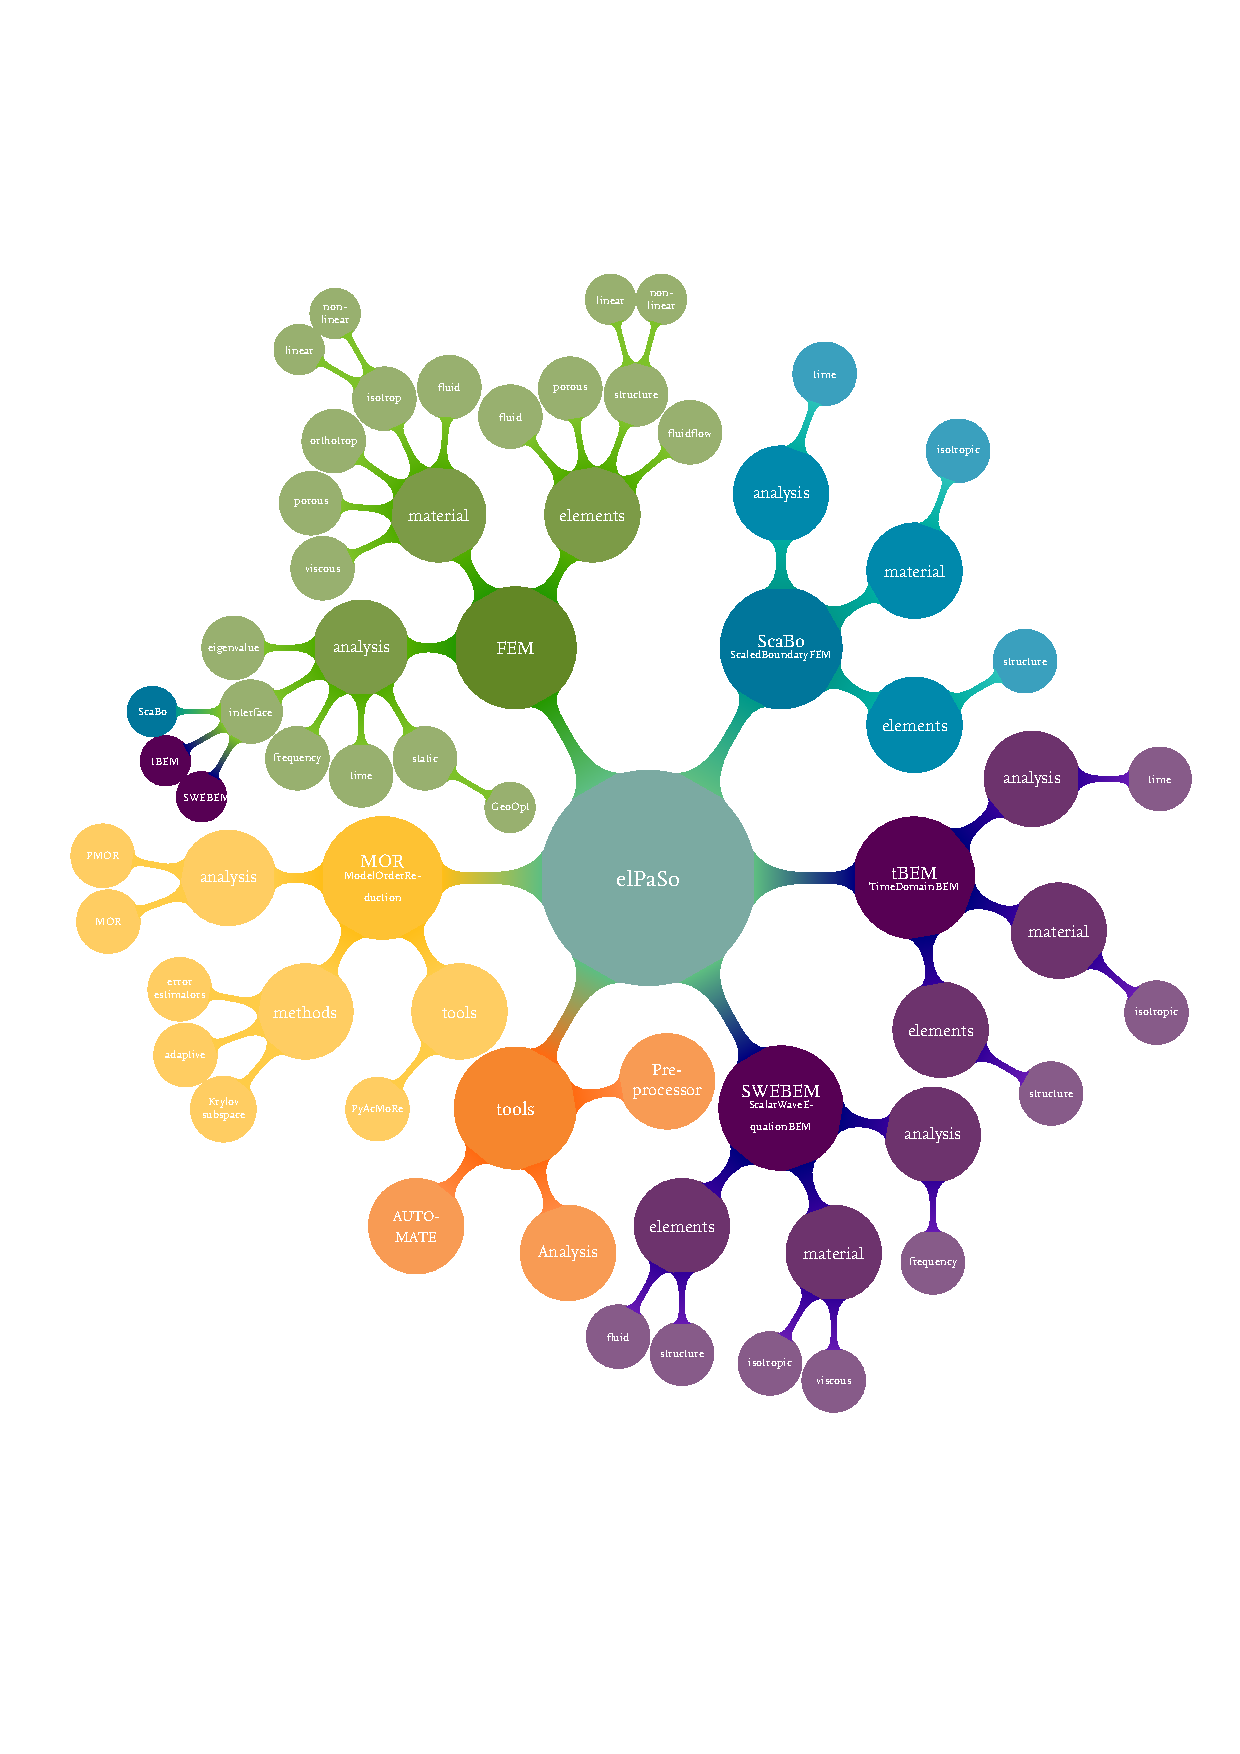
\includegraphics[trim={0 6cm 0 4cm},scale=0.7]{images/elPaSo_bubble.pdf}
    \caption{elPaSo bubble diagram}
\end{figure}

The tool is used extensively for research and teaching for many years. The whole elPaSo project includes the core software written in C++ and other assisting in-house tools written in python. elPaSo offers a wide range of features (see Features and Capability) and facilitates efficient computations in HPC clusters to support parallel computing of large-scale high-fidelity vibroacoustic models. Moreover, the project is built on a flexible and modular framework to support new research features and potential collaborations.

\section{elPaSo Modules}
elPaSo implementations are provided to users and developers in two different modules: (1) \texttt{elPaSo Core (eCore)} module and (2) \texttt{elPaSo Research (eResearch)} module; described as follows.

\subsection{elPaSo Core Module}
The eCore module comprises stable functionalities of elPaSo and is available to the public as open-source. The eCore project can be used as a standalone vibroacoustic simulation tool or/and as a FEM library which can be incorporated into other projects. The main components included in eCore module is discussed in Chapter \ref{chap:eCoreComponents}.

\subsection{elPaSo Research Module}
The eResearch module extends eCore module with advanced features and capabilities. The project is currently closed-source. If you are interested in using or benefitting eResearch functionalities, you are warmly welcome to contact us. A sneak peek into functionalities offered by both the eResearch module is illustrated in Chapter \ref{chap:eCoreComponents}.

\section{Features and Capabilities}

\subsection{Vibroacoustic solver for FEM, BEM and SBFEM}

The capabilities of the tool include acoustic and structural analysis using the popular numerical methods of FEM, BEM and SBFEM supporting various complex material and element types. The solver is suitable for acoustic and structural analysis for static analysis, modal analysis, time domain analysis and frequency domain analysis. Various applied fields with elPaSo are building acoustics, geometric optimizations, wave propagation, soil-structure interactions and fluid-structure interaction.

\subsection{Uncertainty quantification}
elPaSo enables non-intrusive parametric uncertainty quantification (UQ). This capability allows the use of elPaSo as a black-box to obtain the system response associated with each realisation of random vector and UQ is performed as an extension of the deterministic analysis of the model. Also, the possibility to parallelize the elPaSo code in this approach provides an added advantage. These characteristics make the elPaSo solver very attractive for parametric uncertainty quantification in complex models and industrial applications.

\subsection{Model order reduction}
elPaSo provides methods to perform model order reduction in both frequency and parameter domain. As a result, computations can be performed faster in a reduced space without compromising on accuracy. The methods are constantly developed and improved for handling large-scale vibroacoustics models.

\subsection{Code sustainability}
elPaSo ensures code sustainability developed as a part of the DFG project SURESOFT. This includes continuous integration, software testing, containerization and bug reporting. Software-testing concepts in the development workflow incorporating unit-, integration- and performance testing are also adapted within the code. Best practices to facilitate detailed code documentation, both technical and usage, is underway.

\subsection{Efficient deployment}
In order take advantage of the available computational resources, parallel computing has been enabled with MPI and OMP parallelization. elPaSo uses state-of-the-art mathematical routines provided from Intel Math Kernel Library for basic LAPACK and BLAS operations, and PETSc, SLEPc, ARPACK for advanced scientific computations. A wide of direct, iterative and eigen solvers assists the solution process for various analysis types which includes MUMPS, PARDISO and GMRES. The tool is successfully deployed in the TU Braunschweig Phoenix cluster and is used since many years for large-scale computations.

\subsection{Supporting tools and interfaces}
The supporting tools of elPaSo includes sub-projects supporting pre and post processing of simulation data, visualization and advanced computational wrappings. The tools offered are formulated in the following table.

\begin{table}[h!]
    \caption{Overview of supporting tools and interfaces}
    \begin{tabular}{p{8cm}p{8cm}}
    \hline
    \textbf{elPaSo Pre-processor Tool}                                                                                                                                                   & Provides modelling features of material   modelling, loading types, boundary conditions, conforming and non-conforming   coupling interfaces, and many more.                                                                                           \\ \hline
    \textbf{elPaSo Post-processor/Analysis Tool}                                                                                                                                         & Provides a range of post-processing routines to compute the interested   acoustic quantity and routines for visualizing the obtained results. The tool   associates with methods to visualize measurement data and routines to perform   data fitting. \\ \hline
    \textbf{\begin{tabular}[c]{@{}p{8cm}@{}}elPaSo Py-AcMoRe\\    \\ (Python module for faster training and evaluation of vibroacoustics systems using model order reduction)\end{tabular}} & Provides   model order reduction functionalities for faster computations in frequency and parametric domain.                                                                                                                                         \\ \hline
    \end{tabular}
\end{table}

In addition to the above-mentioned in-house tools, elPaSo is open to interface with external softwares. Currently, the code interfaces to commercial softwares of Coreform Cubit and ABAQUS.

\section{Key publications}
\nocite{schauer2012parallel, BLECH2020114960, Sreekumar2021, Sreekumar2023}
\printbibliography[heading=none]
    
\chapter{Components in elPaSo Core}
\label{chap:eCoreComponents}

In this chapter, the main components constituiting the eCore project is described.

\section{Finite element method}
\subsection{Analysis}
\begin{table}[h!]
    \centering
    \caption{Analysis types in elPaSo}
    \begin{tabular}{llcc}
        \hline
        Functionality                                   & Identifier      & elPaSo Core  & elPaSo Research \\ \hline
        Basic frequency domain steady state analysis    & frequency-basic & $\checkmark$ &                 \\
        Advanced frequency domain steady state analysis & frequency       &              & $\checkmark$    \\
        Time domain analysis                            & time            &              & $\checkmark$    \\
        Static analysis                                 & static          &              & $\checkmark$    \\
        Geometrical optimization                        & geoopt          &              & $\checkmark$    \\
        Eigenvalue analysis                             & eigen           &              & $\checkmark$    \\
        Model order reduction                           & mor-offline     &              & $\checkmark$    \\ \hline
    \end{tabular}
\end{table}

\subsection{Elements}

    \begin{longtable}{lcc}
        \hline
        Identifier          & elPaSo Core   & elPaSo Research  \\ \hline
        \multicolumn{3}{c}{Structure   | Beam elements}        \\ \hline
        BeamBernoulli       & $\checkmark$  &                  \\
        BeamTimoshenko      & $\checkmark$  &                  \\
        BeamBernoulli10     & $\checkmark$  &                  \\
        BeamTimoshenko10    & $\checkmark$  &                  \\
        BeamBernoulli12     & $\checkmark$  &                  \\
        BeamTimoshenko12    & $\checkmark$  &                  \\
        BeamBernoulli10nl   &               & $\checkmark$     \\
        BeamTimoshenko10nl  &               & $\checkmark$     \\ \hline
        \multicolumn{3}{c}{Structure | Brick elements}         \\ \hline
        Brick8              & $\checkmark$  &                  \\
        Brick20             &               & $\checkmark$     \\
        Brick27             &               & $\checkmark$     \\ \hline
        \multicolumn{3}{c}{Structure | Plate elements}         \\ \hline
        Kirch4              & $\checkmark$  &                  \\
        DSG3                &               & $\checkmark$     \\
        DSG4                & $\checkmark$  &                  \\
        DSG9                &               & $\checkmark$     \\
        DSG9pre             &               & $\checkmark$     \\ \hline
        \multicolumn{3}{c}{Structure | Disc   elements}        \\ \hline
        Disc3               &               & $\checkmark$     \\
        Disc4               & $\checkmark$  &                  \\
        Disc9               &               & $\checkmark$     \\
        Disc9s              &               & $\checkmark$     \\
        DiscDr4             &               & $\checkmark$     \\ \hline
        \multicolumn{3}{c}{Structure | Shell elements}         \\ \hline
        PlShell3            &               & $\checkmark$     \\
        PlShell4            &               & $\checkmark$     \\
        PlShell9            &               & $\checkmark$     \\
        PlShell9pre         &               & $\checkmark$     \\
        PlShellDr4          &               & $\checkmark$     \\ \hline
        \multicolumn{3}{c}{Structure |   Tetrahedron elements} \\ \hline
        Tetra4              &               & $\checkmark$     \\
        Tetra10             &               & $\checkmark$     \\
        Tetra4L             &               & $\checkmark$     \\
        Tetra10L            &               & $\checkmark$     \\
        Tetra16             &               & $\checkmark$     \\
        Tetra16L            &               & $\checkmark$     \\ \hline
        \multicolumn{3}{c}{Structure | Spring elements}        \\ \hline
        Spring              & $\checkmark$  &                  \\
        Springz             & $\checkmark$  &                  \\ 
        SpringBC            & $\checkmark$  &                  \\ 
        SpringBCx            & $\checkmark$  &                  \\ 
        SpringBCy            & $\checkmark$  &                  \\ 
        SpringBCz            & $\checkmark$  &                  \\
        SpringBCrx            & $\checkmark$  &                  \\ 
        SpringBCry            & $\checkmark$  &                  \\ 
        SpringBCrz            & $\checkmark$  &                  \\ \hline
        \multicolumn{3}{c}{Structure | Point mass}             \\ \hline
        Pointmass           & $\checkmark$  &                  \\ \hline
        \multicolumn{3}{c}{Structure | Cable elements}         \\ \hline
        Cable2D             &               & $\checkmark$     \\
        Cable3D             &               & $\checkmark$     \\ \hline
        \multicolumn{3}{c}{Structure | Porous elements}        \\ \hline
        PoroPlateQ2P1       &               & $\checkmark$     \\
        PoroPlateQ2P2       &               & $\checkmark$     \\
        PoroPlateQ2P3       &               & $\checkmark$     \\
        PoroPlateQ3P1       &               & $\checkmark$     \\
        PoroPlateQ3P3       &               & $\checkmark$     \\
        DiscPQ2P1           &               & $\checkmark$     \\
        ShellQ2P1           &               & $\checkmark$     \\
        PoroPlateKienzler4  &               & $\checkmark$     \\
        PoroDiscKienzler4   &               & $\checkmark$     \\
        PoroShellKienzler4  &               & $\checkmark$     \\
        Poro3dUP8           &               & $\checkmark$     \\
        Poro3dUP27          &               & $\checkmark$     \\
        Poro3dUU8           &               & $\checkmark$     \\ \hline
        \multicolumn{3}{c}{Fluid | Linear elements}            \\ \hline
        Fluid4              &               & $\checkmark$     \\ \hline
        Fluid8              & $\checkmark$  &                  \\ \hline
        Fluid27             &               & $\checkmark$     \\
        Fluid2d4            &               & $\checkmark$     \\
        Fluid2d9            &               & $\checkmark$     \\ \hline
        \multicolumn{3}{c}{Fluid | Flow elements}              \\ \hline
        FF4                 &               & $\checkmark$     \\
        FF9                 &               & $\checkmark$     \\ \hline
        \caption{Element types in elPaSo}
\end{longtable}

\subsection{Materials}
Elpaso is capable of implementing different material models for acoustical simulations. For
example: orthotropic, isotropic, fluid, spring, etc. Each material has its own behavior and
characteristics, each of them being described within the syntax against the respective property
values. See Table \ref{tab:MaterialTypes} for an overview of material types offered in eCore.

\begin{longtable}{p{6cm}p{6cm}cc}
    \hline
    Functionality                                                                                              & Identifier                        & \multicolumn{1}{c}{elPaSo Core} & \multicolumn{1}{c}{elPaSo Research} \\ \hline
    \multicolumn{4}{c}{Structure | Isotropic materials}                                                                                                                                                                    \\ \hline
    Linear elastic isotropic                                                                                   & STR\_LIN\_ELA\_ISO\_DIR           & $\checkmark$                    &                                     \\
    Linear viscoelastic isotropic                                                                              & STR\_LIN\_VIS\_ISO\_DIR           & $\checkmark$                    &                                     \\
    Non-linear elastic isotropic                                                                               & STR\_NL\_ELA\_ISO\_DIR            &                                 & $\checkmark$                        \\
    Linear viscoelastic isotropic   implementing Cremer/Heckl constrained layer damping (CLD) model            & STR\_LIN\_VIS\_ISO\_CLDCH         &                                 & $\checkmark$                        \\
    Linear viscoelastic isotropic   implementing Ross/Kerwin/Ungar (RKU) constrained layer damping (CLD) model & STR\_LIN\_VIS\_ISO\_CLDRKU        &                                 & $\checkmark$                        \\
    Linear viscoelastic isotropic   implementing RKU CLD and laminate theory                                   & STR\_LIN\_VIS\_ISO\_CLDRKU\_LAMWA &                                 & $\checkmark$                        \\\hline
    \multicolumn{4}{c}{Structure |   Orthotropic materials}                                                                                                                                                                \\ \hline
    Linear elastic orthotropic                                                                                 & STR\_LIN\_ELA\_ORT\_DIR           &                                 & $\checkmark$                        \\
    Linear viscoelastic orthotropic                                                                            & STR\_LIN\_VIS\_ORT\_DIR           &                                 & $\checkmark$                        \\
    Linear viscoelastic orthotropic laminate                                                                   & STR\_LIN\_VIS\_ORT\_LAM\_NOPRE    &                                 & $\checkmark$                        \\
    Linear viscoelastic orthotropic laminate   prestressed                                                     & STR\_LIN\_VIS\_ORT\_LAM           &                                 & $\checkmark$                        \\\hline
    \multicolumn{4}{c}{Structure | Spring}                                                                                                                                                                                 \\\hline
    Linear spring orthotropic                                                                                  & STR\_LIN\_SPR\_ORT\_DIR           & $\checkmark$                    &                                     \\\hline
    \multicolumn{4}{c}{Structure | Mass}                                                                                                                                                                                   \\\hline
    Point mass                                                                                                 & STR\_LIN\_POINTMASS               & $\checkmark$                    &                                     \\\hline
    \multicolumn{4}{c}{Fluid | Acoustic}                                                                                                                                                                                   \\\hline
    Linear acoustic fluid undamped                                                                             & AF\_LIN\_UAF\_ISO\_DIR            & $\checkmark$                    &                                     \\
    Linear acoustic fluid damped                                                                               & AF\_LIN\_EQF\_ISO\_DIR            &                                 & $\checkmark$                        \\
    Linear acoustic fluid lossy                                                                                & AF\_LIN\_VIS\_LF\_DIR             &                                 & $\checkmark$                        \\
    Linear acoustic fluid to treat porous   media                                                              & AF\_LIN\_VIS\_ISO\_POROUS         &                                 & $\checkmark$                        \\
    Linear acoustic cloaking fluid                                                                             & AF\_LIN\_CLK\_AISO\_DIR           &                                 & $\checkmark$                        \\\hline
    \multicolumn{4}{c}{Structure |   Poroelastic materials}                                                                                                                                                                \\\hline
    Linear poroelastic                                                                                         & STR\_LIN\_ELA\_POR\_DIR           &                                 & $\checkmark$                        \\
    Linear poroelastic for plate elements   based on Biot's theory                                             & STR\_LIN\_ELA\_POR\_PLATE         &                                 & $\checkmark$                        \\
    Linear poroelastic for foams                                                                               & STR\_LIN\_ELA\_POR\_FOAM          &                                 & $\checkmark$                        \\
    Linear poroelastic 3D elements based on   Biot's theory                                                    & STR\_LIN\_ELA\_POR\_3D            &                                 & $\checkmark$                        \\
    Linear poroelastic 3D elements with loss                                                                   & STR\_LIN\_VIS\_POR\_3D            &                                 & $\checkmark$                        \\
    Linear poroelastic 3D elements with loss   and compression modulus                                         & STR\_LIN\_VIS\_POR\_3DCOMP        &                                 & $\checkmark$                        \\
    Linear poroelastic 3D elements trans                                                                       & STR\_LIN\_ELA\_POR\_3DTRANS       &                                 & $\checkmark$                        \\\hline
    \multicolumn{4}{c}{Structure |   Elasticplatic materials}                                                                                                                                                              \\\hline
    Non-linear elasticplastic cap model                                                                        & STR\_NL\_ELPLA\_ISO\_CM           &                                 & $\checkmark$                        \\
    Non-linear elasticplastic cap model with   outer adjustment                                                & STR\_NL\_ELPLA\_ISO\_CMO          &                                 & $\checkmark$                        \\
    Non-linear elasticplastic Drucker Prager   parameters                                                      & STR\_NL\_ELPLA\_ISO\_DP           &                                 & $\checkmark$                        \\
    Non-linear elasticplastic Drucker Prager   parameters ideal plastic                                        & STR\_NL\_ELPLA\_ISO\_DPIP         &                                 & $\checkmark$                        \\
    Non-linear elasticplastic Drucker Prager   parameters with outer adjustment                                & STR\_NL\_ELPLA\_ISO\_DPO          &                                 & $\checkmark$                        \\
    Non-linear elasticplastic Drucker Prager   parameters with outer adjustment ideal plastic                  & STR\_NL\_ELPLA\_ISO\_DPOIP        &                                 & $\checkmark$                       \\ \hline
    \caption{Material types in elPaSo}
    \label{tab:MaterialTypes}
\end{longtable}

\subsection{Loads}

\begin{table}[H]
    \centering
    \caption{Load types in elPaSo}
    \begin{tabular}{p{6cm}lcc}
        \hline
    Functionality                                                          & Identifier                 & \multicolumn{1}{c}{elPaSo Core} & \multicolumn{1}{c}{elPaSo Research} \\ \hline
    \multicolumn{4}{c}{Nodal loads}                                                                                                                                             \\ \hline
    Force/moment on a node                                                 & point\_force               & $\checkmark$                    &                                     \\
    Force/moment on a node - time dependent                                & structuretime              &                                 & $\checkmark$                        \\
    Sound source at a fluid node                                           & fluid                      & $\checkmark$                    &                                     \\ \hline
    \multicolumn{4}{c}{Element loads}                                                                                                                                           \\ \hline
    Frequency dependent element loads                                      & plane\_wave                &                                 & $\checkmark$                        \\
    Frequency dependent element loads TBL                                  & turbulent\_boundary\_layer &                                 & $\checkmark$                        \\
    Normal velocity vn or flux q acting normal to surface of fluid element & v\_n                       &                                 & $\checkmark$                        \\ \hline
    \end{tabular}
\end{table}

\subsection{Boundary conditions}
\begin{table}[H]
    \centering
    \caption{Boundary condition types in elPaSo}
    \begin{tabular}{llcc}
        \hline
    Functionality                                 & Identifier   & \multicolumn{1}{c}{elPaSo Core} & \multicolumn{1}{c}{elPaSo Research} \\ \hline
    Structural nodal constraints                  & structural   & $\checkmark$                    &                                     \\
    Acoustic nodal constraints                    & acoustic     & $\checkmark$                    &                                     \\
    Acoustic nodal constraints, oblique incidence & fluidoblique &                                 & $\checkmark$                        \\ \hline
    \end{tabular}
    \end{table}

\subsection{Coupling interfaces}

\begin{table}[H]
    \centering
    \caption{Coupling interface types in elPaSo}
    \begin{tabular}{lcc}
        \hline
    Identifier                  & \multicolumn{1}{c}{elPaSo Core} & \multicolumn{1}{c}{elPaSo Research} \\ \hline
    \multicolumn{3}{c}{Conforming interface elements}                                                   \\ \hline
    InterfaceBeam               & $\checkmark$                    &                                     \\
    InterfaceFFPoro3dUP         &                                 & $\checkmark$                        \\
    InterfaceFFShell            &                                 & $\checkmark$                        \\
    InterfaceKirchhoff          & $\checkmark$                    &                                     \\
    InterfaceMindlin            & $\checkmark$                    &                                     \\
    InterfaceMindlinEquiporo    &                                 & $\checkmark$                        \\
    InterfaceMindlinPoro3dUP    &                                 & $\checkmark$                        \\
    InterfacePlaneShellPoro2dUP &                                 & $\checkmark$                        \\
    MultiPointConstraint        &                                 & $\checkmark$                        \\ \hline
    \multicolumn{3}{c}{Non-conforming interface elements}                                               \\ \hline
    NCInterfaceMindlin          &                                 & $\checkmark$                        \\
    NCInterfaceMindlinEquiporo  &                                 & $\checkmark$                        \\ \hline
    \end{tabular}
    \end{table}

\section{Input file definition}
Input to elPaSo is currently limited to tailor-made HDF5 file format produced by the elPaSo Preprocessing tool. Support for other common file formats is in development. However, you can develop a new parser to support your input file by adapting from the parser interface class in cFemParserInterface.h. Contact us if you require support.

\section{Output file formats}
Various output file formats are support for outputting simulation results. Currently eCore supports HDF5, VTK and STP.
\chapter{Using elPaSo Core}

As already mentioned in the introduction, elPaSo Core is can be used in two ways according to your purpose:
\begin{enumerate}
    \item \textbf{eCore Executable}: The executable can be used to solve vibroacoustic problems. Guideline to compile an elpaso executable is outlined in Section \ref{sec:eCoreAsSolver}.
    \item \textbf{eCore Library}: By generating eCore library, you can link eCore as a third party library in your project and use the FEM functionalies from eCore.
\end{enumerate}

\section{elPaSo Core as a vibroacoustic solver} \label{sec:eCoreAsSolver}

elPaSo can be with GNU compilers and Intel compilers (recommended). This section mainly focus on elPaSo preparation using a basic GNU compiler.

\subsection{Executable types}
\begin{enumerate}
    \item \textbf{elpaso}: Executable compiled with real data-types and hence computations without complex domain (mainly used for time-domain computations).
    \item \textbf{elpasoC}: Executable compiled with complex data type.
    \item \textbf{elpasoT}: Executable running all the unit-tests for eCore using GoogleTest.
\end{enumerate}

\subsection{Building executable}
\begin{enumerate}
    \item Download and run the docker image containing the basic environment required for building elPaSo. This contains the necessary third part libraries and compiler.
    \begin{itemize}
        \item \texttt{sudo docker pull <link to the image will follow soon after intial release>}
        \item \texttt{sudo docker run -it <image name>}
        \item Now you are inside the container with all necessary elPaSo dependencies.
    \end{itemize}
    \item Checkout the current version of the elPaSo Core project
    \begin{itemize}
        \item \texttt{git clone https://git.rz.tu-bs.de/akustik/elPaSo-Core}
        \item \texttt{cd elPaSo-Core}
    \end{itemize}
    \item Configure a cmake configuration file for your system
    \begin{itemize}
        \item \texttt{make cmake-gen}
        \item This creates a config.cmake file with your hostname in the "cmake" folder. The file contains the default configuration. You need not change anything here unless required.
    \end{itemize}
    \item Build elPaSo Core executable
    \begin{enumerate}
        \item With GNU compiler
        \begin{itemize}
            \item \texttt{mkdir project}
            \item \texttt{make elpaso-gnu}
            \item \texttt{make elpaso-build}
            \item When sucessfull, executables (elpaso, elpasoC and elpasoT) are generated in ./bin folder. 
        \end{itemize}
        \item With Intel compiler
        \begin{itemize}
            \item Install intel-parallel-studio and configure the ./cmake/\$HOSTNAME.config.cmake with the respective directory where the installation is done with INTEL\_DIR and the respective version number to INTELMPI\_VERSION.
            \item \texttt{mkdir project}
            \item \texttt{make elpaso-intel}
            \item \texttt{make elpaso-build}
            \item Executables (elpaso, elpasoC and elpasoT) are generated in ./bin folder. 
        \end{itemize}
    \end{enumerate}
\end{enumerate}

\subsection{Running executable}
elPaSo can be started by direct use of the compiled files elpaso and elpasoC. The input file is
needed in the folder where the calculation is started. A simple serial run with standard settings
can be made by the command: \\

{\hspace{2em} \tt elpasoC -c -inp myInputFile.hdf5}\\

A check of the input file is started by the command: \\

{\hspace{2em} \tt elpasoC -check -inp myInputFile.hdf5}\\

To run problems with the executable elpaso having real-only petsc datatype, follow the same commands with the respective executable name: \\

{\hspace{2em} \tt elpaso -c -inp myInputFile.hdf5}\\

Unit-tests can be performed by running the test executable: \\

{\hspace{2em} \tt elpasoT}\\

\subsection{Running executable in parallel using MPI}
In order to execute elpaso in parallel may some additional MPI commands have to be used. These commands
are depending on the computer used, e.g.,\\

{\hspace{2em} \tt mpirun -np 4 elpasoC -c -inp myInputFile.hdf5}\\

in order to run the program using 4 processes. \texttt{mpirun} is the instance supplied from an MPI vendor. For GNU compiler build, we use OpenMPI and for INTEL compiler build, we use Intel MPI.

\section{elPaSo Core as a FEM library} \label{sec:eCoreAsLibrary}
\subsection{Building library}

\begin{enumerate}
    \item Download and run the docker image containing the basic environment required for building elPaSo. This contains the necessary third part libraries and compiler.
    \begin{itemize}
        \item \texttt{sudo docker pull <link to the image will follow soon after intial release>}
        \item \texttt{sudo docker run -it <image name>}
        \item Now you are inside the container with all necessary elPaSo dependencies.
    \end{itemize}
    \item Checkout the current version of the elPaSo Core project
    \begin{itemize}
        \item \texttt{git clone https://git.rz.tu-bs.de/akustik/elPaSo-Core}
        \item \texttt{cd elPaSo-Core}
    \end{itemize}
    \item Configure a cmake configuration file for your system
    \begin{itemize}
        \item \texttt{make cmake-gen}
        \item This creates a config.cmake file with your hostname in the "cmake" folder. The file contains the default configuration.
        \item To generate the eCore library, active the library generation option in ./cmake/\$HOSTNAME.config.cmake by modifying: \texttt{OPTION(GEN\_DLIB			"elPaSo DYNAMIC LIB"	ON)}
    \end{itemize}
    \item Build elPaSo Core library
    \begin{enumerate}
        \item With GNU compiler
        \begin{itemize}
            \item \texttt{mkdir project}
            \item \texttt{make elpaso-gnu}
            \item \texttt{make elpasolib-build}
            \item When sucessfull, elpasoCore-gnu folder contains the necessary entities for linking eCore.
        \end{itemize}
        \item With Intel compiler
        \begin{itemize}
            \item Install intel-parallel-studio and configure the ./cmake/\$HOSTNAME.config.cmake with the respective directory where the installation is done with INTEL\_DIR and the respective version number to INTELMPI\_VERSION.
            \item \texttt{mkdir project}
            \item \texttt{make elpaso-intel}
            \item \texttt{make elpasolib-build}
            \item When sucessfull, elpasoCore-intel folder contains the necessary entities for linking eCore.
        \end{itemize}
    \end{enumerate}
\end{enumerate}

\subsection{Linking library}
Follow the steps below, to link eCore library with CMake. In your FindELPASOCORE.cmake:
\begin{enumerate}
    \item Include the path \texttt{./elpasoCore-<COMPILER>/include} to your cmake project for link to header files
    \item Link the eCore dynamic library:
    \begin{itemize}
        \item For real-valued build, link \texttt{./elpasoCore-<COMPILER>/lib/libelpasoCore-intel-cxx-o.so}
        \item For complex-valued build, link \texttt{./elpasoCore-<COMPILER>/lib/libelpasoCore-intel-cxx-complex.so}
    \end{itemize}
\end{enumerate}
%\chapter{Using elPaSo Core}

\end{document}